%! Author = adam
%! Date = 28.02.21


\chapter{Particle Accelerators}\label{ch:particle-accelerators}
So we have a source of ions, now we wish to accelerate those ions towards a sample.
There are a few main components of an accelerator, but the main concept involves using electric fields (since we have charged particles).
To ensure that these accelerated particles actually travel to a sample, we could use a closed evacuated beam-line system (a vacuum in which the particles travel) with pressure of around $10^{-5} $ mbar.
The particles need to be guided, so a deflection system consisting of an electrical beam is necessary, but also can be implemented using focussing elements like magnetic lenses.
While the ion beam is travelling, we might want to also be able to measure the beam position/current, so detectors would be nice to have in an accelerator.
Apertures, like those in a camera, could ensure a good beam quality.
Of course radiation protection equipment is necessary, but this will not be talked about so much.

There are basically two types of accelerators, and a few examples of each are given in the table below:
\begin{center}
\begin{tabular}{ c | c }
	\hline
	Electrostatic Accelerators & AC Accelerators \\
	\hline
	Van-de-Graaff / Pelletron & Cyclotron \\
	Cockcroft-Walton & Linear Acc (LINAC) \\
	& Synchrotron
\end{tabular}
\end{center}

\section{Electrostatic Accelerators}\label{sec:electrostatic-accelerators}
These were the first type of accelerators discovered and used, as they are quite simple, and much cheaper to use.
Additionally, they deliver a continuous beam, which is not possible with AC accelerators (pulsed beam), and this continuous beam then leads to a high beam current, resulting in a very 'industry friendly' accelerator.
The electrostatic accelerators can further be divided into two groups, single ended vs tandem machines.
The general design of an electrostatic accelerator is given in Figure~\ref{fig:eagen}.

\begin{figure}
	\centering
	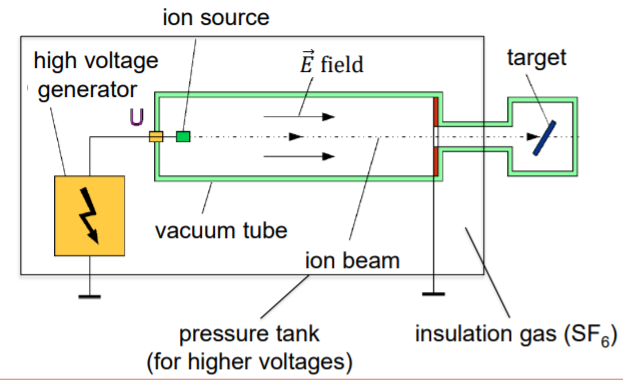
\includegraphics[width = 0.8\linewidth, height = 5cm]{general_acc_pic}
	\caption{The basic overview of ES accelerators. Surrounding the accelerator, we have a grounded insulation gas (typically SF$_6$ for its high pressure) tank, because in the vacuum chamber we will produce a very high electric field and the voltage generators will carry high voltages (several million Volts) to the ion source. The danger of breaking through the vacuum tube is high, so the insulation gas helps prevent any of these breakthroughs. The electric field moves the ions generated by the ion source.}
	\label{fig:eagen}
\end{figure}

\subsection{Single Ended Machines}\label{subsec:single-ended-machines}
\begin{wrapfigure}{r}{0.5\linewidth}
	\centering
	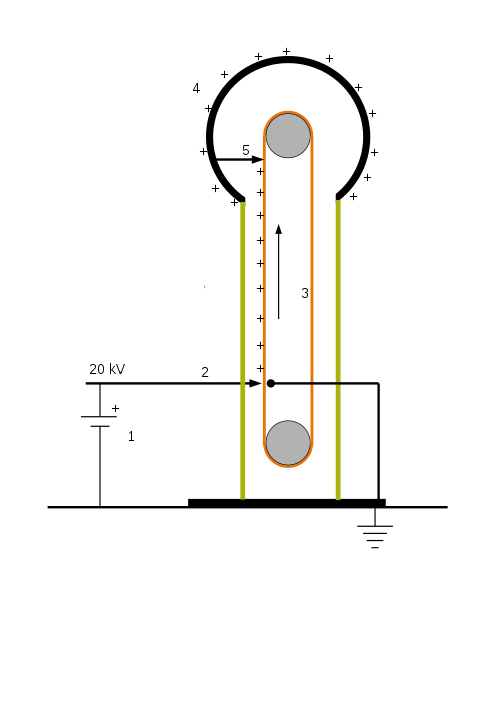
\includegraphics[scale=0.15]{degraff}
	\caption{Van-de-Graaf Generator}
	\label{fig:degraff}
\end{wrapfigure}
Incredibly high voltages are needed to produce ions for electrostatic accelerators, so we need a transformer, and one idea is to use Van-de-Graaf generators.
A 'spray' voltage brings positive charges onto an insulated charge belt (normally rubber), which transports the charges to a 'charge remover point'.
The charges are then positively charging the pressure tank, where they are able to push out the positive ion sources (same charges repel each other).
A simple equation determines the voltage in the pressure tank, $U = \frac{Q}{C}$ where $Q$ is the charges and $C$ is the capacitance of the tank apparatus.
This tank is the same as the desk experiment from high school, where you touch your hands on the big metal ball and your hair pushed up.
The first Van-de-Graff generator was 12 meters high, but with big height came with a big punch as it could generate around 5 million volts!

Nowadays, we use a similar idea, called the pelletron.
Instead of an insulating rubber band chain that carriers the positive charges, the Pelletron uses a chain with small metal segments in between.
This allows the accelerator to be charged much faster since charges are transported much faster on metal than they are on rubber bands.
For a more sophisticated approach to produce high voltages, we could use the Cockcroft-Walton high voltage cascade, which even in 1932, one could produce 700 keV protons using this method.
By alternating capacitors in a ladder like way, one is able to steadily increase the voltage, while using diodes to prevent the charges from flowing backwards.
The capacitors store up charge based on the previous capacitors plus the initial voltage.
So if we have a starting max voltage of an AC charge of 100V, and we had 4 levels of ladder, we would get a resulting voltage of 400 V.
There are no mechanical parts for this, which means less maintenance.
For each type of single ended machine discussed, the resulting energy of the ions produced is given by the equation $E_i = qU$ where $q$ is the charge of the ion, and $U$ is the potential energy of the electric field produced to accelerate the ions.

\subsection{Tandem Machines}\label{subsec:tandem-machines}

Up to now we have discussed single ended machines for accelerating ions, but now we will discuss tandem machines.
The name comes from the fact that the voltage we use to accelerate the ions is used twice.
Contrary to the single ended machine, the ion source is on ground for tandem machines.
The ions coming into the device are negatively charged, meaning that the electric field in the tank will push particles towards the center of the tank.
Then in the middle of the tank, there is what is called a 'gas stripper', and the electrons are removed from the ion, resulting in positively charged ions, which are then pushed in the same direction they were previously traveling.
A schematic is given in Figure~\ref{fig:tandem}.
The downside to this method is this gas stripper, which will 'dull' the beam, and our change in energy from the gas stripper is high.
So the beam current will not be so nice if we throw away low energy ions.
\begin{figure}
	\centering
	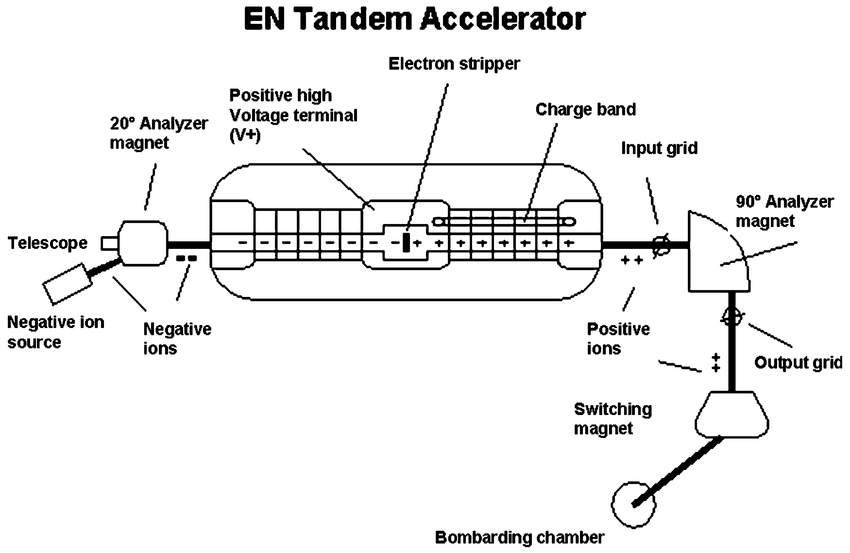
\includegraphics[width=0.8\linewidth, height=5.5cm]{Tandem-accelerator}
	\caption{The basic overview of the tandem ion accelerator. The potential is used two times. The two magnets at each end are diagnostic purposes, where we can select which ions we want to use for the ion beam. Voltages for the supply are normally around $10 MW$ resulting in 20 MeV energies. }
	\label{fig:tandem}
\end{figure}



\section{AC Accelerators}\label{sec:ac-accelerators}
AC Accelerators have an advantage over ES accelerators, which has to do with the insulation issue.
In ES systems, the insulation tanks are there to protect from catastrophe, thus limiting the voltages from becoming higher than a few mega volts.
However, AC do not have this limitation.
Also a big distinction between AC and DC accelerators is the type of ion beam produced.
For AC accelerators, we use pulsed currents (hence AC), such that the ions are not a constant flow (like in DC), but rather periodic (like a laser pulse).

\subsection{Cyclotrons}\label{subsec:cyclotrons}

There are over 2000 cyclotrons spread across the world, and have applications like the production of radio nuclide in medicine.
An examination of cyclotrons can be found in Chapter 4, section 4.1 where we discuss ion beam transport.
Applying a radio frequency range AC voltage ( $\omega = \frac{qB}{2\pi m}$) with a magnetic field perpendicular to the applied voltage, there will be a Lorentz force, guiding the particle in a circular path.
The radio frequency is set so that the particle makes one circuit during one period of this frequency $\omega$.
The velocity will increase with each path between the gaps of these 'dees'.
In the 'dees' it is a Faraday cup essentially.
On the end of one of the 'dees' there is a voltage plate used to deflect the particle into the beam line.
We can calculate using maxwell equations to find what energies are possible.
The centripetal force must be equal to the force of the magnetic field. $$ F_c = F_B \rightarrow \frac{mv^2}{r} = qvB \Rightarrow v = \frac{qBr}{m}$$
We can see that at $r \rightarrow R$ where $R$ is maximum radius of the device,\[ v = \frac{qBR}{m}\] and the maximum energy of the particle is given by
\[E_{\max} = \frac{1}{2} mv^2 \Rightarrow \frac{1}{2} \frac{(qBR)^2}{m} \]
This typically results in ion energy values of 10--500 MeV! This is much higher than the energies in electrostatic accelerators.
The problem with this is that it can be very expensive to create a large machine, and the size of the machine depends heavily on the resulting energy of the ion.
We must also take into account relativistic effects, so the frequency $\omega$ becomes $\frac{\omega_0}{\gamma} = \omega_0 \sqrt{1 - \beta^2} $, where $\beta = \frac{v}{c}$ and $\omega_0$ is the non-relativistic frequency defined above.
Because of these relativistic factor, it is not useful to use the electron, as relativistic effects occur at very low energies, whereas for high mass particles, the relativistic effects are not so apparent at useful energies.

\subsection{Betatron}\label{subsec:betatron}
In a Betatron, the changing magnetic field from the primary coil accelerates electrons injected into a vacuum torus, causing them to circle around the torus, in the same manner as current induced in the second coil of a transform.
The primary factor is a stable orbit, which satisfies the following equation:
\[\theta_0 = 2\pi r_0^2 H_0\]
where $\theta_0$ is the flux within the area enclosed by the electron orbit, $r_0$ is the radius of the electron orbit, $H_0$ is the magnetic field at $r_0$.
This means that the magnetic field at the orbit must be half the average magnetic field over its circular cross section, a condition called Wideroes condition:
\[ H_0 = \frac{1}{2}\frac{\theta_0}{\pi r_0^2} \]
This method is not used these days, but originally were used to produce electron beams up to 300 MeV.
The maximum energy is limited by the strength of the magnetic field, due to the saturation of iron and size of magnet core.
Synchrotron overcame these limitations.

\subsection{LINAC}\label{subsec:linac}
The linear accelerator starts with an ion source, followed by many 'drift tubes' in a linear connection.
Each drift tube is connected to an RF generator, so that each time an ion is between the tubes, the amplitude of the RF voltage is positive whereas in the drift tube it is negative, leading the drift tube to be a faraday cage.
The acceleration is thus between the connections of the tubes, and the length of the drift tubes need to be increased for each acceleration step.
All in all the length of each tube is based on the frequency of the driving voltage of the RF generator, as well as which particles you want to accelerate.
If we assume a constant frequency, then the period of time it takes to go through one of the drift tube, $L_n$, must be half of the frequency $f$ (particle is always accelerated in the gaps).
Wolf Widerue derived the condition for the drift tube lengths $l_n$, which is as follows: The energy of an particle being accelerated after the $n$th drift tube is given by
$$ E_n = qUn $$
where $U$ is the amplitude of the AC voltage.
This, in the classical case, is equal to
\[ E_n = \frac{m}{2}v_n^2 = \frac{m}{2} \left(\frac{l_n}{L_n}\right)^2 \rightarrow l_n = \frac{1}{f}\sqrt{\frac{nqU}{2m}} \]
The factor $L_n$ is the characteristic half period, also given by $L_n=\frac{1}{2}\frac{1}{f}$.
As we can see, with the mass being in the denominator of the equation above, for very small particles (like electrons), we need very long tube lengths if we want high energies.
It is important to note also that since we use an RF generator, we are using pulsed beams.


\section{Summary}\label{sec:summary}

\begin{myitemize}
	\item Once ions are generated we need to accelerate them, and there are two main methods to this: AC and Electrostatic
	\item Electrostatic is the cheapest and most industry friendly, and is divided into two methods, single ended vs tandem
	\item tandem machines rely on negatively charged ions, and result in high energies but not so good beam current
	\item single ended machines are generally good, can be done without the use of mechanical parts via the Cockcraft-Walton cascade
	\item AC accelerators produce ion energies much greater than the ES approach (10-100 MeV)
\end{myitemize}

